% ====================================================================
% v7-07b.tex -- graphite anode dQ/dV ICA theory Chapter 1, v7-07b
% Source spine: AUTHOR_BRIEF.md, v11_flowchart.md, Anode_Fit_v11_final.py, graphite_ica_ch1_Opus_v5.tex.
% ====================================================================
\documentclass[11pt,a4paper]{article}
\usepackage[margin=22mm]{geometry}
\usepackage{kotex}
\setmonofont{D2Coding}[Scale=MatchLowercase]
\usepackage{amsmath,amssymb,mathtools,bm}
\usepackage{booktabs,longtable,array}
\usepackage{enumitem}
\usepackage{amsthm}
\usepackage{hyperref}
\usepackage{fancyhdr}
\usepackage{lastpage}
\usepackage{setspace}
\usepackage{tikz}
\usetikzlibrary{positioning,arrows.meta}
\setstretch{1.12}
\setlength{\parskip}{0.45em}
\setlength{\parindent}{0pt}
\setlength{\headheight}{14pt}
\setlength{\emergencystretch}{2em}
\hypersetup{colorlinks=true, linkcolor=blue, urlcolor=blue, citecolor=blue,
  pdftitle={Graphite anode dQ/dV theory Chapter 1 v7-07b}}
\pagestyle{fancy}\fancyhf{}
\lhead{흑연 음극 $dQ/dV$ 이론 -- Ch.1 v7-07b}\rhead{\thepage/\pageref{LastPage}}
\renewcommand{\headrulewidth}{0.4pt}

\newtheorem*{keybox}{핵심}
\newtheorem*{verifybox}{검산}
\newtheorem*{guardbox}{운용 조건}

\newcommand{\dd}{\mathrm{d}}
\newcommand{\app}{\mathrm{app}}
\newcommand{\cellc}{\mathrm{cell}}
\newcommand{\cell}{\mathrm{cell}}
\newcommand{\bg}{\mathrm{bg}}
\newcommand{\eq}{\mathrm{eq}}
\newcommand{\eff}{\mathrm{eff}}
\newcommand{\hys}{\mathrm{hys}}
\newcommand{\dis}{\mathrm{dis}}
\newcommand{\chg}{\mathrm{chg}}
\newcommand{\work}{\mathrm{work}}
\newcommand{\rep}{\mathrm{rep}}
\newcommand{\peak}{\mathrm{peak}}
\newcommand{\lag}{\mathrm{lagged}}

\renewcommand{\theequation}{1.\arabic{equation}}
\renewcommand{\thesection}{1.\arabic{section}}

\title{\textbf{\LARGE Chapter 1}\\[0.35em]\Large 흑연 음극 $dQ/dV$ 이론: v11\_final 계산 순서의 수식 유도}
\author{}
\date{}

\begin{document}
\maketitle

\section*{서론}
\addcontentsline{toc}{section}{서론}
이 문건은 \texttt{GraphiteAnodeDischargeDQDV.dqdv} 가 한 곡선을 계산하는 순서 그대로 흑연 음극 ICA 식을 닫는다. 공유 spine 의 노드 순서는 N0 에서 N9 까지다. 전개는 수식이 주도한다. 산문은 앞 절의 출력이 다음 절의 입력으로 넘어가는 다리만 맡는다.

코드의 반환량은 관측 격자 $V_\app$ 위의 미분용량이다.
\begin{equation}
\boxed{\;\frac{\dd Q}{\dd V_\app}(V_\app;T,|I|,Q_\cell,\sigma_d)\;}
\label{eq:target}
\end{equation}
여기서 방향 부호는
\begin{equation}
\sigma_d=\begin{cases}
+1,&\text{방전}\\
-1,&\text{충전}
\end{cases}
\label{eq:sigmadef}
\end{equation}
이다. 방전은 음극 탈리튬화이자 산화로 둔다. 방전에서는 $V$ 증가가 탈리튬화 진행률 증가와 같은 방향이다. 충전에서는 진행 방향이 전압 격자의 감소 방향이므로 N8 에서 격자 역전이 필요하다.

\begin{figure}[t]
\centering
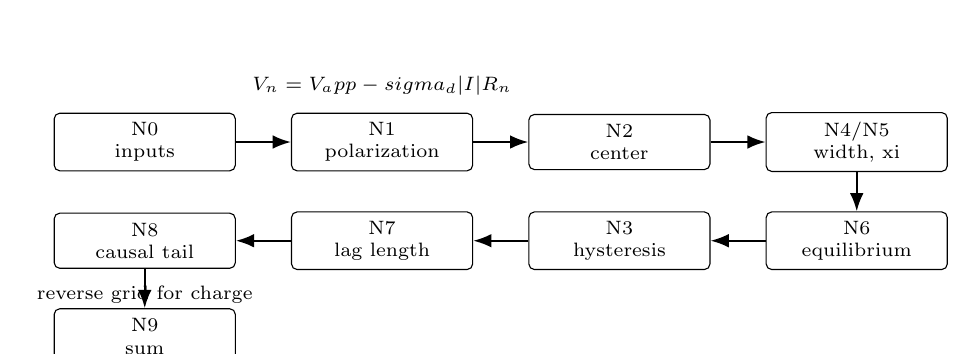
\begin{tikzpicture}[
  node distance=5mm and 7mm,
  box/.style={draw,rounded corners=2pt,minimum width=23mm,minimum height=7mm,align=center,font=\scriptsize},
  arr/.style={-Latex,thick}
]
\node[box] (n0) {N0\\inputs};
\node[box,right=of n0] (n1) {N1\\polarization};
\node[box,right=of n1] (n2) {N2\\center};
\node[box,right=of n2] (n4) {N4/N5\\width, xi};
\node[box,below=of n4] (n6) {N6\\equilibrium};
\node[box,left=of n6] (n3) {N3\\hysteresis};
\node[box,left=of n3] (n7) {N7\\lag length};
\node[box,left=of n7] (n8) {N8\\causal tail};
\node[box,below=of n8] (n9) {N9\\sum};
\draw[arr] (n0) -- (n1);
\draw[arr] (n1) -- (n2);
\draw[arr] (n2) -- (n4);
\draw[arr] (n4) -- (n6);
\draw[arr] (n6) -- (n3);
\draw[arr] (n3) -- (n7);
\draw[arr] (n7) -- (n8);
\draw[arr] (n8) -- (n9);
\node[font=\scriptsize,above=1mm of n1] {$V_n=V_app-sigma_d |I| R_n$};
\node[font=\scriptsize,below=1mm of n8] {reverse grid for charge};
\end{tikzpicture}
\caption{v11\_final 계산 순서의 문서 spine. 그림 안의 텍스트는 ASCII 만 사용했다. N3 의 히스테리시스는 코드 호출 위치가 N2 뒤이지만, 문서에서는 평형 peak 를 먼저 닫은 뒤 분기 중심이 peak 위치를 어떻게 바꾸는지 설명한다. 본문 전개는 이 그림의 순서를 따른다.}
\label{fig:spine}
\end{figure}

그림~\ref{fig:spine} 의 각 상자는 코드 식별자 하나 또는 작은 함수 묶음에 대응한다. 최종 합산은 \texttt{dqdv\_work += tr['Q'] * peak\_shape} 와 \texttt{np.interp} 로 닫힌다.

\tableofcontents
\newpage

% ====================================================================
\section{N0: 실험조건에서 모델 입력으로}\label{sec:n0}
% ====================================================================
상위 facade \texttt{curve} 는 실험 라벨을 core 인자로 바꾼다. 방향 문자열은 \texttt{\_direction\_to\_sigma} 로 식~\eqref{eq:sigmadef} 에 매핑되고, 전류 크기는
\begin{equation}
|I|=\begin{cases}
\texttt{I\_abs},&\texttt{I\_abs}\ \text{가 주어질 때}\\
\texttt{c\_rate}\,Q_\cell,&\texttt{I\_abs}\ \text{가 없을 때}
\end{cases}
\label{eq:Iabs}
\end{equation}
로 결정된다. core 함수의 입력은
\begin{equation}
\texttt{dqdv}(V_\app,T,|I|,Q_\cell,s=\sigma_d)
\label{eq:dqdvcall}
\end{equation}
이다. 용량 좌표는
\begin{equation}
q=\frac{Q}{Q_\cell},\qquad \frac{\dd q}{\dd t}=\frac{|I|}{Q_\cell}
\label{eq:qdef}
\end{equation}
이며, 관측량은 식~\eqref{eq:target} 이다.

전이 집합은 \texttt{transitions} 의 원소 $j=1,\dots,N_p$ 이다. 각 원소는
\begin{equation}
\{U,w,n,Q,\Omega,\gamma,h_\eta,\Delta H_{\mathrm{rxn}},\Delta S_{\mathrm{rxn}},\Delta H_a,\Delta S_a,\dd V/\dd q|_{q_a},L_V\}
\label{eq:trdict}
\end{equation}
중 필요한 키를 가진다. \texttt{GRAPHITE\_STAGING\_LIT} 의 초기값은 표~\ref{tab:staging} 에 정리했다.

\begin{table}[t]
\centering
\renewcommand{\arraystretch}{1.25}
\begin{tabular}{lrrrrrrr}
\toprule
전이 & $U$ [V] & $w$ [V] & $Q$ & $\Omega$ [J/mol] & $\Delta H_{\mathrm{rxn}}$ & $\Delta S_{\mathrm{rxn}}$ & $\Delta H_a$\\
\midrule
stage $4\to3$ & 0.210 & 0.020 & 0.10 & 6000 & -11700 & +29 & 48000\\
stage $3\to2L$ & 0.140 & 0.016 & 0.12 & 8000 & -13500 & 0 & 46000\\
stage $2L\to2$ & 0.120 & 0.014 & 0.25 & 10000 & -13100 & -5 & 44000\\
stage $2\to1$ & 0.085 & 0.012 & 0.50 & 13000 & -13000 & -16 & 40000\\
\bottomrule
\end{tabular}
\caption{\texttt{GRAPHITE\_STAGING\_LIT} 초기값. 모든 값은 피팅 시작점이며, \texttt{dVdq\_qa}=0.30, \texttt{dS\_a}=0.0 이 네 전이에 공통으로 들어간다.}
\label{tab:staging}
\end{table}

N0 의 출력은 $\sigma_d,|I|,T,Q_\cell,V_\app,\{tr_j\}$ 이다. N1 은 이 중 $V_\app,\sigma_d,|I|,R_n$ 만 써서 내부 전위 격자를 만든다.

% ====================================================================
\section{N1: 분극 보정과 작업 격자}\label{sec:n1}
% ====================================================================
측정 전위와 내부 음극 전위는 lumped 저항 $R_n$ 으로 연결된다. v11\_final 의 정본 식은
\begin{equation}
\boxed{\;V_n=V_\app-\sigma_d|I|R_n\;}
\label{eq:polarization}
\end{equation}
이다. 방전 $\sigma_d=+1$ 에서 관측 전위 $V_\app$ 에는 분극 상승분이 들어 있으므로, 열역학 전위는 이를 뺀 $V_n$ 이다. 충전 $\sigma_d=-1$ 에서는 부호가 반대라 $V_n=V_\app+|I|R_n$ 이 된다.

\begin{verifybox}
분극 부호 검산:
\begin{equation}
V_\app=V_n+\sigma_d|I|R_n
\quad\Longleftrightarrow\quad
V_n=V_\app-\sigma_d|I|R_n.
\label{eq:polarcheck}
\end{equation}
방전 peak 의 관측 위치는 내부 중심보다 $|I|R_n$ 만큼 높다. 충전 peak 의 관측 위치는 내부 중심보다 $|I|R_n$ 만큼 낮다. 관측 gap 에서는 두 분극이 더해져 $2|I|R_n$ 이 된다.
\end{verifybox}

꼬리 합성곱은 입력 격자보다 넓은 작업 격자에서 계산된다.
\begin{align}
v_{\min}&=\min V_n,\qquad v_{\max}=\max V_n,\qquad
\Delta v=\max(v_{\max}-v_{\min},\texttt{v\_span\_floor}),\label{eq:vspan}\\
N_{\work}&=\max(\texttt{n\_work\_min},\,2|V_n|),\label{eq:nwork}\\
V_{\work}&=\operatorname{linspace}(v_{\min}-\texttt{grid\_pad\_lo}\,\Delta v,\,
v_{\max}+\texttt{grid\_pad\_hi}\,\Delta v,\,N_{\work}),\label{eq:vwork}\\
\Delta V_{\work}&=V_{\work,i+1}-V_{\work,i}.
\label{eq:gridstep}
\end{align}
온도 입력이 배열이면 $V_n$ 정렬 후 $V_{\work}$ 위로 보간하고, 스칼라면 $T_{\work}=T\mathbf 1$ 이다. 대표 온도는
\begin{equation}
T_{\rep}=\operatorname{mean}(T_{\work})
\label{eq:Trep}
\end{equation}
이다. 배경은
\begin{equation}
C_\bg(V_{\work})=
\begin{cases}
\texttt{Cbg}(V_{\work}),&\texttt{Cbg}\ \text{가 callable}\\
\texttt{Cbg}\,\mathbf 1,&\texttt{Cbg}\ \text{가 scalar}
\end{cases}
\label{eq:Cbg}
\end{equation}
로 시작 배열 \texttt{dqdv\_work} 에 들어간다.

N1 의 출력은 $V_n,V_{\work},\Delta V_{\work},T_{\work},T_{\rep},C_\bg$ 이다. N2 는 전이별 평형 중심 $U_j(T)$ 를 계산한다.

% ====================================================================
\section{N2: 평형 중심 $U_j(T)$}\label{sec:n2}
% ====================================================================
평형 전위는 반응 Gibbs 자유에너지에서 나온다. 반쪽전지 전위의 정의를
\begin{equation}
\Delta G_j(T)=-F\,U_j(T)
\label{eq:gibbsU}
\end{equation}
로 두고, 상압 등온 항등식
\begin{equation}
\Delta G_j(T)=\Delta H_{\mathrm{rxn},j}-T\Delta S_{\mathrm{rxn},j}
\label{eq:gibbsHS}
\end{equation}
를 대입하면
\begin{equation}
\boxed{\;U_j(T)=\frac{-\Delta H_{\mathrm{rxn},j}+T\Delta S_{\mathrm{rxn},j}}{F}\;}
\label{eq:UjT}
\end{equation}
이다. 이는 \texttt{func\_U\_j(T,dH\_rxn,dS\_rxn)} 와 1:1 대응한다.

전이 dict 가 \texttt{dH\_rxn} 과 \texttt{dS\_rxn} 을 모두 가지면 식~\eqref{eq:UjT} 를 배열 $T_{\work}$ 에 적용한다. 그렇지 않으면 직접 입력된 \texttt{U} 를 쓴다.
\begin{equation}
U_j=\begin{cases}
\texttt{func\_U\_j}(T_{\work},\texttt{dH\_rxn},\texttt{dS\_rxn}),&
\texttt{dH\_rxn,dS\_rxn}\in tr_j\\
\texttt{U},&\text{그 외}
\end{cases}
\label{eq:Uchoice}
\end{equation}

\begin{verifybox}
부호 검산:
\begin{equation}
\frac{\partial U_j}{\partial T}=\frac{\Delta S_{\mathrm{rxn},j}}{F}.
\label{eq:dUdT}
\end{equation}
$\Delta H_{\mathrm{rxn}}<0$ 인 흑연 staging 초기값은 $-\Delta H_{\mathrm{rxn}}>0$ 이므로 양의 전위 중심을 준다. $T=298.15$ K 에서 stage $4\to3$ 의 중심은 $[11700+298.15(29)]/96485\simeq0.211$ V 로 표~\ref{tab:staging} 의 $0.210$ V 와 맞는다.
\end{verifybox}

N2 의 출력은 전이별 $U_j(T_{\work})$ 또는 상수 $U_j$ 이다. N4 와 N5 는 이 중심 주변의 폭과 점유율을 닫는다.

% ====================================================================
\section{N4--N5: 폭과 평형 점유율}\label{sec:n4n5}
% ====================================================================
먼저 폭이다. 코드 기본 폭은 \texttt{func\_w} 다.
\begin{equation}
\boxed{\;w_j(T)=\frac{n_jRT}{F}\;}
\label{eq:w}
\end{equation}
\texttt{\_n\_factor} 는 dict 키의 우선순위를 다음처럼 둔다.
\begin{equation}
n_j(T)=
\begin{cases}
\texttt{n},&\texttt{n}\ \text{이 주어질 때}\\
\texttt{w}\,F/(RT),&\texttt{w}\ \text{가 주어질 때}\\
1,&\text{그 외}
\end{cases}
\label{eq:nfactor}
\end{equation}
\texttt{use\_w\_eff=True} 이고 $\Omega_j$ 가 있으며 직접 \texttt{w} 가 없을 때는 정규용액 중심 기울기의 유효 폭을 쓴다.
\begin{align}
w_j^{\eff}(T)&=\frac{RT}{F}\left(1-\frac{\Omega_j}{2RT}\right),\label{eq:weffraw}\\
w_j^{\eff,\mathrm{clip}}(T)&=\max\left[w_j^{\eff}(T),\,\texttt{w\_eff\_floor\_frac}\frac{RT}{F}\right].
\label{eq:weffclip}
\end{align}
식~\eqref{eq:weffraw}--\eqref{eq:weffclip} 은 \texttt{func\_w\_eff(T,Omega,floor\_frac)} 와 1:1 대응한다.
따라서 \texttt{\_width} 의 출력은
\begin{equation}
w_j=
\begin{cases}
w_j^{\eff,\mathrm{clip}},&
\texttt{use\_w\_eff}\land(\Omega_j\ \text{있음})\land(\texttt{w}\ \text{없음})\\
n_jRT/F,&\text{그 외}
\end{cases}
\label{eq:widthchoice}
\end{equation}
이다.

이제 점유율이다. 이 절에서 전위 의존성은 무차원 driving coordinate 로만 쓴다. 기호 $A_j$ 는 N7 의 코드 컷 affinity 상수에 예약한다. 정방향과 역방향 속도의 detailed balance 는
\begin{equation}
\frac{r_j^+}{r_j^-}=\exp(z_j),
\qquad
\quad z_j=\frac{\sigma_d(V-U)}{w_j}
\label{eq:dbv7}
\end{equation}
를 요구한다. 정지점에서는 $r_j^+(1-\xi)=r_j^-\xi$ 이므로
\begin{align}
\frac{\xi_{\eq,j}}{1-\xi_{\eq,j}}
&=\exp\!\left[\frac{\sigma_d(V-U)}{w_j}\right].
\label{eq:logit}
\end{align}
따라서 코드 \texttt{func\_ksi\_eq} 의 식은
\begin{equation}
\boxed{\;\xi_{\eq,j}(V,T,U,w,\sigma_d)=
\frac{1}{1+\exp[-z_j]},\qquad
z_j=\frac{\sigma_d(V-U)}{w_j}\;}
\label{eq:xieq}
\end{equation}
이다. overflow 를 피하려고 코드는 $z\ge0$ 과 $z<0$ 를 나눠 같은 logistic 값을 계산한다.

\begin{figure}[t]
\centering
\begin{tikzpicture}[x=1.2cm,y=3.3cm]
\draw[->] (-4.4,0) -- (4.5,0) node[below] {$sigma_d (V-U) / w$};
\draw[->] (-4.4,0) -- (-4.4,1.15) node[above] {$xi_eq$};
\draw[thick] plot[smooth] coordinates {(-4,0.018) (-3,0.047) (-2,0.119) (-1,0.269) (0,0.5) (1,0.731) (2,0.881) (3,0.953) (4,0.982)};
\draw[densely dashed,thick] plot[smooth] coordinates {(-4,0.0177) (-3,0.0452) (-2,0.105) (-1,0.1966) (0,0.25) (1,0.1966) (2,0.105) (3,0.0452) (4,0.0177)};
\node[font=\scriptsize] at (2.7,0.82) {xi\_eq};
\node[font=\scriptsize] at (2.4,0.20) {xi(1-xi)};
\draw[dotted] (0,0) -- (0,1.02);
\node[font=\scriptsize,below] at (0,0) {center};
\end{tikzpicture}
\caption{logistic 점유율과 그 미분 핵. 본문 식~\eqref{eq:xieq} 와 식~\eqref{eq:dxidVv7} 의 시각화다. 방전과 충전은 $sigma_d(V-U)$ 축에서 같은 모양을 갖는다.}
\label{fig:logistic}
\end{figure}

그림~\ref{fig:logistic} 은 식~\eqref{eq:xieq} 의 방향 불변 모양을 보여준다. N6 은 이 logistic 을 미분해 평형 peak 를 얻는다.

% ====================================================================
\section{N6: 평형 peak와 \texttt{equilibrium}}\label{sec:n6}
% ====================================================================
$z_j=\sigma_d(V_n-U_j)/w_j$ 로 놓으면
\begin{align}
\frac{\dd \xi_{\eq,j}}{\dd z_j}
&=\frac{e^{-z_j}}{(1+e^{-z_j})^2}
=\xi_{\eq,j}(1-\xi_{\eq,j}),\label{eq:dxidz}\\
\frac{\dd z_j}{\dd V_n}
&=\frac{\sigma_d}{w_j}.
\label{eq:dzdV}
\end{align}
따라서
\begin{equation}
\frac{\dd\xi_{\eq,j}}{\dd V_n}
=\frac{\sigma_d\,\xi_{\eq,j}(1-\xi_{\eq,j})}{w_j}.
\label{eq:dxidVv7}
\end{equation}
ICA peak 는 방향에 관계없이 양수 크기로 더해야 하므로 코드의 평형 기여는
\begin{equation}
\boxed{\;\texttt{peak\_shape}_{j,\eq}
=\frac{\xi_{\eq,j}(1-\xi_{\eq,j})}{w_j}\;}
\label{eq:eqpeakv7}
\end{equation}
이다. 이는 \texttt{equilibrium(V\_n,T)} 의 내부 루프
\begin{equation}
\texttt{dqdv}\leftarrow C_\bg+\sum_j Q_j\frac{\xi_{\eq,j}(1-\xi_{\eq,j})}{w_j}
\label{eq:equilibrium}
\end{equation}
와 일치한다. 중심, 높이, 면적은
\begin{equation}
V_{\peak,j}=U_j,\qquad
\left(\frac{\dd Q}{\dd V}\right)_{\max,j}^{\mathrm{net}}=\frac{Q_j}{4w_j},\qquad
\int Q_j\frac{\xi_{\eq,j}(1-\xi_{\eq,j})}{w_j}\,\dd V=Q_j
\label{eq:eqprops}
\end{equation}
이다.

\begin{verifybox}
방전에서는 $\sigma_d=+1$ 이므로 $V_n$ 증가가 $\xi_{\eq}$ 증가를 만든다. 충전에서는 $\sigma_d=-1$ 이므로 $V_n$ 증가가 충전 진행률 기준의 $\xi_{\eq}$ 감소를 만든다. 그러나 식~\eqref{eq:eqpeakv7} 는 부호를 제거한 peak 크기라 항상 양수다.
\end{verifybox}

N6 까지는 히스테리시스가 없는 평형 중심을 기준으로 했다. N3 은 같은 peak 식의 중심을 방향별 분기 중심으로 바꾼다.

% ====================================================================
\section{N3: 히스테리시스 분기 중심}\label{sec:n3}
% ====================================================================
정규용액 자유에너지를 진행률 $\xi$ 로 쓰면
\begin{equation}
g_j(\xi)=g_j^0+RT\{\xi\ln\xi+(1-\xi)\ln(1-\xi)\}+\Omega_j\xi(1-\xi).
\label{eq:gxi_v7}
\end{equation}
두 번 미분하면
\begin{equation}
g_j''(\xi)=\frac{RT}{\xi(1-\xi)}-2\Omega_j.
\label{eq:gpp_v7}
\end{equation}
spinodal 은 $g_j''=0$ 의 해다.
\begin{equation}
\xi_{s,j}^{\pm}=\frac12\pm\frac12u_j,\qquad
u_j=\sqrt{1-\frac{2RT}{\Omega_j}},\qquad \Omega_j>2RT.
\label{eq:spinodal_v7}
\end{equation}
$\Omega_j\le2RT$ 에서는 실수 spinodal 이 없고 gap 을 0 으로 둔다.

평형 전위의 비상수 항은 logit 항과 상호작용 항이다.
\begin{equation}
V_{\eq,j}(\xi)=U_j+\frac{RT}{F}\ln\frac{\xi}{1-\xi}
+\frac{\Omega_j}{F}(1-2\xi)
\label{eq:Veq_v7}
\end{equation}
여기서 두 항 사이의 $+$ 는 중요하다. logit 항과 상호작용 항은 각각 같은 식 안의 독립 기여이며, 누락되면 다음 spinodal 차가 식~\eqref{eq:dUhysraw} 로 이어지지 않는다.

spinodal 좌표를 식~\eqref{eq:spinodal_v7} 에서
\begin{equation}
\xi_+=\frac{1+u_j}{2},\qquad
\xi_-=\frac{1-u_j}{2}
\label{eq:spinodalpm}
\end{equation}
로 쓰면 각 끝점의 logit 과 상호작용 항은
\begin{align}
\ln\frac{\xi_+}{1-\xi_+}&=2\operatorname{artanh}u_j,
&
1-2\xi_+&=-u_j,\label{eq:spinodalplus}\\
\ln\frac{\xi_-}{1-\xi_-}&=-2\operatorname{artanh}u_j,
&
1-2\xi_-&=u_j.\label{eq:spinodalminus}
\end{align}
따라서 두 끝점 전위는
\begin{align}
V_{\eq,j}(\xi_+)
&=U_j+\frac{2RT}{F}\operatorname{artanh}u_j-\frac{\Omega_j}{F}u_j,\label{eq:Vspinplus}\\
V_{\eq,j}(\xi_-)
&=U_j-\frac{2RT}{F}\operatorname{artanh}u_j+\frac{\Omega_j}{F}u_j.\label{eq:Vspinminus}
\end{align}
히스테리시스 폭은 낮은 점유율 쪽 spinodal 전위에서 높은 점유율 쪽 spinodal 전위를 뺀 양수 gap 으로 둔다.
\begin{align}
\Delta U_j^\hys
&=V_{\eq,j}(\xi_-)-V_{\eq,j}(\xi_+)\notag\\
&=\frac{2}{F}\left[\Omega_j u_j-2RT\,\operatorname{artanh}u_j\right],
\qquad u_j=\sqrt{1-\frac{2RT}{\Omega_j}},\label{eq:dUhysraw}\\
\Delta U_j^\hys&=0,\qquad \Omega_j\le2RT.
\label{eq:dUhyszero}
\end{align}
이는 \texttt{func\_dU\_hys(T,Omega)} 와 1:1 대응한다.

실측 분기는 spinodal 상한을 축소 인자 $\gamma_j$ 와 부분 cycle 인자 $h_\eta$ 로 안쪽으로 당긴다. v11\_final 의 분기 중심은
\begin{equation}
\boxed{\;U_j^d=U_j+\frac12\,\sigma_d\,h_\eta\,\gamma_j\,\Delta U_j^\hys\;}
\label{eq:Ubranch}
\end{equation}
이다. 이는 \texttt{func\_U\_branch(T,U\_j,Omega,gamma,sigma\_d,h\_eta)} 와 일치한다.

\begin{figure}[t]
\centering
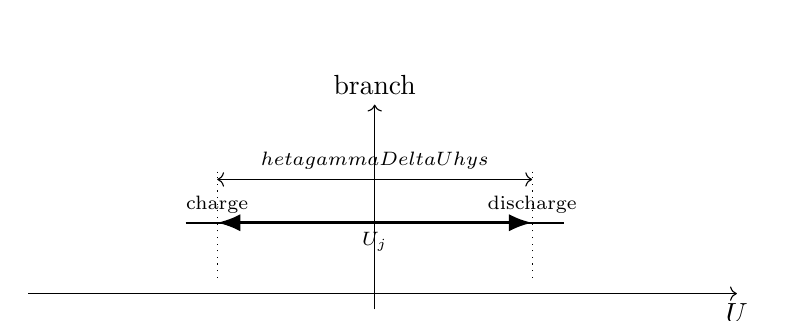
\begin{tikzpicture}[x=2.0cm,y=1.0cm]
\draw[->] (-2.2,0) -- (2.3,0) node[below] {$U$};
\draw[->] (0,-0.2) -- (0,2.4) node[above] {branch};
\draw[thick] (-1.2,0.9) -- (1.2,0.9);
\draw[very thick,-Latex] (0,0.9) -- (1.0,0.9);
\draw[very thick,-Latex] (0,0.9) -- (-1.0,0.9);
\node[font=\scriptsize,below] at (0,0.9) {$U_j$};
\node[font=\scriptsize,above] at (1.0,0.9) {discharge};
\node[font=\scriptsize,above] at (-1.0,0.9) {charge};
\draw[<->] (-1.0,1.45) -- (1.0,1.45) node[midway,above,font=\scriptsize] {$h eta gamma Delta U hys$};
\draw[dotted] (-1.0,0.2) -- (-1.0,1.55);
\draw[dotted] (1.0,0.2) -- (1.0,1.55);
\end{tikzpicture}
\caption{분기 중심의 방향 이동. 방전 중심은 $U_j$ 위쪽, 충전 중심은 $U_j$ 아래쪽에 놓이며 총 간격은 $h_\eta\gamma_j\Delta U_j^\hys$ 이다.}
\label{fig:hysbranch}
\end{figure}

그림~\ref{fig:hysbranch} 의 방향 이동은 식~\eqref{eq:polarization} 의 관측 분극과 별개다. 내부 중심 gap 은 $h_\eta\gamma_j\Delta U_j^\hys$ 이고, 관측 peak gap 은 여기에 $2|I|R_n$ 이 더해진다.

N3 의 출력은 \texttt{center} 다.
\begin{equation}
\texttt{center}_j=
\begin{cases}
U_j+\texttt{func\_U\_branch}(T_{\rep},0,\Omega_j,\gamma_j,\sigma_d,h_\eta),&
\gamma_j\ne0,\ \Omega_j>0\\
U_j,&\text{그 외}
\end{cases}
\label{eq:centerchoice}
\end{equation}
N5 의 logistic 은 $U$ 자리에 이 \texttt{center} 를 넣어 평가된다. N7 은 같은 전이에 동역학 지연 길이를 붙인다.

% ====================================================================
\section{N7: Eyring--BV 동역학과 지연 길이}\label{sec:n7}
% ====================================================================
꼬리 길이는 요구 속도와 완화 속도의 비다.
\begin{equation}
L_{q,j}=\frac{|I|}{Q_\cell k_j}.
\label{eq:Lqbasic}
\end{equation}
Eyring 식은
\begin{equation}
k_0=\frac{k_BT}{h},\qquad
\Delta G_{a,j}=\Delta H_{a,j}-T\Delta S_{a,j}
\label{eq:eyringv7}
\end{equation}
이다. 전위 의존 driving force 를 먼저 $\Phi_j(V)$ 로 쓰면
\begin{equation}
\Phi_j(V)=\sigma_dF\!\left[V_n-U_j^d\right]
\label{eq:drivingphi}
\end{equation}
이다. 이는 위치별 장벽을 설명하는 중간 변수일 뿐이며, v11 코드의 컷 affinity 기호 $A_j$ 와 구분한다. \texttt{\_resolve\_lag\_length} 는 실제 지연 길이를 위치별로 다시 계산하지 않고 전이당 대표 컷점에서 한 번 평가한다.
\begin{equation}
\boxed{\;A_j=\min\{\texttt{z\_cut}\,n_jRT,\ \texttt{A\_cap\_RT}\,RT\}\;}
\label{eq:Acut}
\end{equation}
따라서 $A_j$ 는 전이당 상수이며 $V_{\work}$ 와 무관하다. 전위 의존성은 식~\eqref{eq:drivingphi} 의 driving-force 해석에만 남고, 코드 계산형에서는 컷 대표값 $A_j$ 로 동결된다.

컷 대표값에서 BV 장벽 이동은
\begin{equation}
k_j=k_0\exp\!\left[-\frac{\Delta G_{a,j}^{\eff}-\chi_d A_j}{RT}\right]\left(1+e^{-A_j/RT}\right).
\label{eq:kv7}
\end{equation}
\texttt{z\_cut}=4.357 은 logistic 원천 기울기가 정점의 약 $5\%$ 로 떨어지는 위치에 해당한다.

방향별 전달계수는 \texttt{func\_chi\_d} 이다.
\begin{equation}
\boxed{\;\chi_d=
\begin{cases}
\chi,&\sigma_d\ge0\\
1-\chi,&\sigma_d<0
\end{cases}\;}
\label{eq:chid}
\end{equation}
상호작용이 깊은 꼬리의 상수 장벽 몫으로 흡수되면
\begin{equation}
\boxed{\;\Delta H_{a,j}^{\eff}=\Delta H_{a,j}-\chi_d\Omega_j\;}
\label{eq:dHaeff}
\end{equation}
이다. 이는 \texttt{func\_dH\_a\_eff(dH\_a,Omega,chi\_d)} 와 대응한다. \texttt{use\_dH\_eff=False} 이면 코드가 $\Delta H_{a,j}^{\eff}=\Delta H_{a,j}$ 를 쓴다.

식~\eqref{eq:Lqbasic}--\eqref{eq:kv7} 를 대입하면 코드 \texttt{func\_L\_q} 의 식이 단계적으로 나온다.
\begin{align}
L_{q,j}
&=\frac{|I|}{Q_\cell}
\left[
\frac{k_BT}{h}
\exp\!\left(-\frac{\Delta G_{a,j}^{\eff}-\chi_dA_j}{RT}\right)
\left(1+e^{-A_j/(RT)}\right)
\right]^{-1}\notag\\
&=\frac{|I|h}{Q_\cell k_BT}
\frac{\exp[(\Delta G_{a,j}^{\eff}-\chi_dA_j)/(RT)]}
{1+\exp[-A_j/(RT)]}\notag\\
&=
\boxed{\;L_{q,j}=
\frac{|I|h}{Q_\cell k_BT}
\frac{\exp[(\Delta H_{a,j}^{\eff}-T\Delta S_{a,j}-\chi_d A_j)/(RT)]}
{1+\exp[-A_j/(RT)]}\;}
\label{eq:Lqcode}
\end{align}
코드는 \texttt{T\_attempt=(I/Q\_cell)h/kB} 를 만든 뒤 식~\eqref{eq:Lqcode} 의 로그를 평가한다.

전압축 길이는
\begin{equation}
\boxed{\;L_{V,j}=|\dd V_n/\dd q|_{q_a}\,L_{q,j}\;}
\label{eq:LV}
\end{equation}
이며 dict 키는 \texttt{dVdq\_qa} 이다. dict 에 \texttt{L\_V} 가 직접 있으면 \texttt{\_resolve\_lag\_length} 는 동역학 계산을 우회하고 그 값을 쓴다. $|I|\le0$ 이거나 \texttt{dH\_a} 가 없으면 $L_{V,j}=0$ 이다.

전위가 올라갈 때 꼬리가 짧아지는 부호는 컷으로 동결하기 전의 driving force $\Phi_j(V)$ 에 대한 로그 미분으로 확인된다. forward 창에서 분모의 역방향 항은 부호 판단을 바꾸지 않고, 장벽 항은
\begin{equation}
\frac{\partial\ln L_{q,j}}{\partial V}
=-\frac{\chi_d\sigma_dF}{RT}.
\label{eq:dlnLdVraw}
\end{equation}
진행 방향 좌표 $\sigma_dV$ 에 대해서는
\begin{equation}
\frac{\partial\ln L_{q,j}}{\partial(\sigma_dV)}
=-\frac{\chi_dF}{RT}<0.
\label{eq:dlnLdV}
\end{equation}
따라서 방전에서 $V$ 증가가 장벽을 낮추고 꼬리를 짧게 한다. 충전에서도 진행 방향으로 보면 같은 부호가 유지된다. 코드의 $A_j$ 는 이 해석을 전이당 컷 대표점에서 평가한 상수다.

N7 의 출력은 전이별 상수 \texttt{lag\_len\_V} 다. N8 은 이 길이가 격자보다 충분히 큰 경우에만 인과 기억 필터를 켠다.

% ====================================================================
\section{N8: 인과 기억 꼬리와 충전 격자 역전}\label{sec:n8}
% ====================================================================
평형 목표 $\xi_{\eq}$ 를 유한 속도로 따라가는 1차 완화식은
\begin{equation}
\frac{\dd \xi_j}{\dd q}=\frac{\xi_{\eq,j}-\xi_j}{L_{q,j}}.
\label{eq:relaxqv7}
\end{equation}
지연을 $r_j=\xi_{\eq,j}-\xi_j$ 로 두면
\begin{equation}
\frac{\dd r_j}{\dd q}=\frac{\dd \xi_{\eq,j}}{\dd q}-\frac{r_j}{L_{q,j}}.
\label{eq:rv7}
\end{equation}
상수 $L_{q,j}$ 구간의 해는 지수 기억이다.
\begin{equation}
r_j(q)=r_j(q_0)e^{-(q-q_0)/L_{q,j}}
+\int_{q_0}^{q}e^{-(q-q')/L_{q,j}}
\frac{\dd\xi_{\eq,j}}{\dd q'}\,\dd q'.
\label{eq:memoryv7}
\end{equation}
식~\eqref{eq:memoryv7} 의 $+$ 는 외부 forcing $\dd\xi_{\eq}/\dd q$ 가 지연 $r$ 을 생성한다는 항이다. 빠지면 완화항만 남아 peak 꼬리가 원천 변화에서 만들어지지 않는다.

코드는 $r$ 을 직접 적분하지 않고, 같은 1차 완화식을 지연 점유율 $\bar\xi$ 에 적용한다. 전압 진행 좌표에서
\begin{equation}
\frac{\dd\bar\xi_j}{\dd V}=\frac{\xi_{\eq,j}-\bar\xi_j}{L_{V,j}}
\label{eq:lowpassode}
\end{equation}
이고, 한 격자 구간에서 $\xi_{\eq}$ 를 오른쪽 샘플값 $\xi_{\eq,j,i}$ 로 고정하면
\begin{align}
\bar\xi_j(V_i)-\xi_{\eq,j,i}
&=\left[\bar\xi_j(V_{i-1})-\xi_{\eq,j,i}\right]
\exp\!\left(-\frac{\Delta V_{\work}}{L_{V,j}}\right),\label{eq:lowpasssolve}\\
\bar\xi_{j,i}
&=\alpha_j\bar\xi_{j,i-1}+(1-\alpha_j)\xi_{\eq,j,i}.
\label{eq:lowpassderived}
\end{align}
따라서 전압 격자에서 \texttt{\_causal\_lowpass} 의 재귀식은
\begin{align}
\alpha_j&=\exp\!\left(-\frac{\Delta V_{\work}}{L_{V,j}}\right),\label{eq:alpha}\\
\bar\xi_{j,0}&=\xi_{\eq,j,0},\label{eq:initlag}\\
\bar\xi_{j,i}&=\alpha_j\bar\xi_{j,i-1}+(1-\alpha_j)\xi_{\eq,j,i}.
\label{eq:lowpass}
\end{align}
코드에서 $\bar\xi$ 는 \texttt{occ\_lagged} 다.

방전에서는 진행 방향이 $V_{\work}$ 오름차순이다.
\begin{equation}
\bar\xi_j=\texttt{\_causal\_lowpass}(\xi_{\eq,j},\Delta V_{\work},L_{V,j}),\qquad \sigma_d\ge0.
\label{eq:dislowpass}
\end{equation}
충전에서는 진행 방향이 $V_{\work}$ 내림차순이다. 따라서 코드가 배열을 뒤집어 필터링한 뒤 다시 뒤집는다.
\begin{equation}
\bar\xi_j=
\left[\texttt{\_causal\_lowpass}(\xi_{\eq,j}^{\mathrm{rev}},\Delta V_{\work},L_{V,j})\right]^{\mathrm{rev}},
\qquad \sigma_d<0.
\label{eq:chglowpass}
\end{equation}

\begin{figure}[t]
\centering
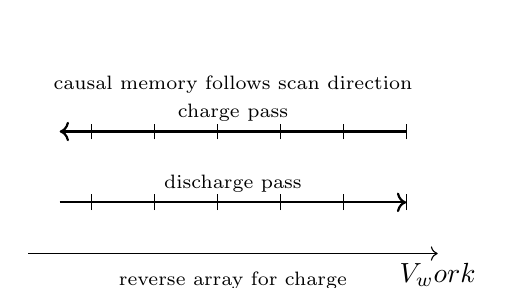
\begin{tikzpicture}[x=1.0cm,y=1.0cm]
\draw[->] (0,0) -- (5.2,0) node[below] {$V_work$};
\draw[->,thick] (0.4,0.65) -- (4.8,0.65) node[midway,above,font=\scriptsize] {discharge pass};
\draw[->,thick] (4.8,1.55) -- (0.4,1.55) node[midway,above,font=\scriptsize] {charge pass};
\foreach \x in {0.8,1.6,2.4,3.2,4.0,4.8} {
  \draw (\x,0.55) -- (\x,0.75);
  \draw (\x,1.45) -- (\x,1.65);
}
\node[font=\scriptsize] at (2.6,2.15) {causal memory follows scan direction};
\node[font=\scriptsize] at (2.6,-0.35) {reverse array for charge};
\end{tikzpicture}
\caption{충전 격자 역전 규칙. 같은 오름차순 작업 격자라도 인과 과거는 scan 방향으로 정의되므로 충전은 배열을 뒤집어 필터링해야 한다.}
\label{fig:tailreverse}
\end{figure}

그림~\ref{fig:tailreverse} 의 역전이 없으면 충전 꼬리가 미래를 참조한다. 이는 인과성과 충방전 거울 양수 peak 조건을 동시에 깨는 부호 결함이다.

지연이 sub-grid 이면 평형 peak 를 쓴다.
\begin{equation}
L_{V,j}<\texttt{min\_lag\_grid\_steps}\,\Delta V_{\work}
\quad\Longrightarrow\quad
\texttt{peak\_shape}_j=\frac{\xi_{\eq,j}(1-\xi_{\eq,j})}{w_j}.
\label{eq:minlag}
\end{equation}
그렇지 않으면 코드의 꼬리 peak 는
\begin{equation}
\boxed{\;\texttt{peak\_shape}_j=\frac{\xi_{\eq,j}-\bar\xi_j}{L_{V,j}}\;}
\label{eq:tailshape}
\end{equation}
이다. $L_{V,j}\to0$ 극한에서는 저역통과가 항등에 가까워지며 식~\eqref{eq:minlag} 의 평형 peak 로 환원한다.

N8 의 출력은 \texttt{peak\_shape} 다. N9 는 이를 전이 용량 $Q_j$ 로 가중 합산한다.

% ====================================================================
\section{N9: 합산, 역보간, 피팅 가능 사양}\label{sec:n9}
% ====================================================================
전하 보존식은 서로소 전이 용량과 배경 용량의 합이다.
\begin{equation}
Q(V_n)=Q_\bg(V_n,T)+\sum_{j=1}^{N_p}Q_j\xi_j(V_n).
\label{eq:chargev7}
\end{equation}
궤적을 따라 미분하면
\begin{equation}
\frac{\dd Q}{\dd V_n}=C_\bg(V_n,T)+\sum_{j=1}^{N_p}Q_j\frac{\dd\xi_j}{\dd V_n}.
\label{eq:sumgeneric}
\end{equation}
v11\_final 의 계산형은 이 미분을 작업 격자에서 직접 쌓는다.
\begin{equation}
\boxed{\;\texttt{dqdv\_work}
=C_\bg(V_{\work})+\sum_{j=1}^{N_p}Q_j\,\texttt{peak\_shape}_j\;}
\label{eq:dqdvwork}
\end{equation}
여기서
\begin{equation}
\texttt{peak\_shape}_j=
\begin{cases}
\xi_{\eq,j}(1-\xi_{\eq,j})/w_j,&
L_{V,j}<\texttt{min\_lag\_grid\_steps}\,\Delta V_{\work}\\[3pt]
(\xi_{\eq,j}-\bar\xi_j)/L_{V,j},&\text{그 외}
\end{cases}
\label{eq:peakchoice}
\end{equation}
이다. 마지막 반환은 입력 내부 전위 $V_n$ 으로 역보간한다.
\begin{equation}
\boxed{\;\frac{\dd Q}{\dd V_\app}(V_\app)
=\operatorname{interp}\{V_n;\,V_{\work},\,\texttt{dqdv\_work}\}\;}
\label{eq:interp}
\end{equation}
식~\eqref{eq:polarization} 의 $V_n=V_\app-\sigma_d|I|R_n$ 이 이미 적용되어 있으므로 반환 배열은 원래 $V_\app$ 격자와 같은 shape 을 가진다.

\begin{keybox}
v11\_final 을 재현하는 최소 구현 순서:
\begin{enumerate}[leftmargin=2.0em,itemsep=1pt]
\item \texttt{curve} 에서 direction 을 $\sigma_d$ 로, C-rate 를 $|I|$ 로 바꾼다.
\item 식~\eqref{eq:polarization} 으로 $V_n$ 을 만들고 식~\eqref{eq:vwork} 의 작업 격자를 만든다.
\item \texttt{Cbg} 로 \texttt{dqdv\_work} 를 초기화한다.
\item 각 전이에서 식~\eqref{eq:Uchoice}, 식~\eqref{eq:centerchoice}, 식~\eqref{eq:widthchoice}, 식~\eqref{eq:xieq} 를 순서대로 계산한다.
\item 식~\eqref{eq:Acut}, 식~\eqref{eq:chid}, 식~\eqref{eq:dHaeff}, 식~\eqref{eq:Lqcode}, 식~\eqref{eq:LV} 로 \texttt{lag\_len\_V} 를 얻는다.
\item 식~\eqref{eq:minlag} 또는 식~\eqref{eq:tailshape} 로 \texttt{peak\_shape} 를 정한다. 충전이면 식~\eqref{eq:chglowpass} 의 격자 역전을 적용한다.
\item 식~\eqref{eq:dqdvwork} 로 합산하고 식~\eqref{eq:interp} 로 입력 격자에 되돌린다.
\end{enumerate}
\end{keybox}

피팅 실행에 필요한 하이퍼파라미터와 dict 키는 표~\ref{tab:codeids} 에 모았다.
\begin{table}[t]
\centering
\renewcommand{\arraystretch}{1.25}
\begin{tabular}{p{0.24\textwidth} p{0.34\textwidth} p{0.30\textwidth}}
\toprule
코드 식별자 & 수식 위치 & 역할\\
\midrule
\texttt{Rn} & \eqref{eq:polarization} & 관측 전위에서 내부 전위를 복원하는 lumped 저항\\
\texttt{grid\_pad\_lo, grid\_pad\_hi} & \eqref{eq:vwork} & 꼬리 필터가 경계에서 잘리지 않도록 작업 격자 확장\\
\texttt{n\_work\_min} & \eqref{eq:nwork} & 합성곱 격자 최소 해상도\\
\texttt{v\_span\_floor} & \eqref{eq:vspan} & 스칼라 또는 좁은 입력의 0 span 방지\\
\texttt{z\_cut} & \eqref{eq:Acut} & logistic 원천이 정점의 약 $5\%$ 로 떨어지는 affinity 컷\\
\texttt{A\_cap\_RT} & \eqref{eq:Acut} & 컷 affinity 상한\\
\texttt{min\_lag\_grid\_steps} & \eqref{eq:minlag} & sub-grid 꼬리를 평형 peak 로 환원하는 문턱\\
\texttt{chi\_split} & \eqref{eq:chid} & 기본값은 \texttt{func\_chi\_d}; 사용자 callable 로 교체 가능\\
\texttt{use\_dH\_eff} & \eqref{eq:dHaeff} & $\Omega$ 의 장벽 흡수 적용 여부\\
\texttt{use\_w\_eff} & \eqref{eq:weffclip} & 정규용액 폭 좁힘 적용 여부\\
\bottomrule
\end{tabular}
\caption{v11\_final 식별자와 수식 대응. 표의 식별자는 코드 spelling 을 보존했다.}
\label{tab:codeids}
\end{table}

\begin{verifybox}
부호 사슬 최종 검산:
\begin{align}
U_j(T)&=(-\Delta H_{\mathrm{rxn}}+T\Delta S_{\mathrm{rxn}})/F,\label{eq:sign1}\\
\xi_{\eq}&=\operatorname{logistic}[\sigma_d(V_n-U)/w],\label{eq:sign2}\\
\frac{\dd\xi_{\eq}}{\dd V_n}&=\sigma_d\xi_{\eq}(1-\xi_{\eq})/w,\qquad
\texttt{peak\_shape}_{\eq}=\xi_{\eq}(1-\xi_{\eq})/w>0,\label{eq:sign3}\\
\Delta U^\hys&\ge0,\qquad U_j^d=U_j+\frac12\sigma_dh_\eta\gamma\Delta U^\hys,\label{eq:sign4}\\
\chi_d&=\chi\ \text{방전},\qquad \chi_d=1-\chi\ \text{충전},\label{eq:sign5}\\
\Delta H_a^\eff&=\Delta H_a-\chi_d\Omega,\label{eq:sign6}\\
\partial\ln L_q/\partial(\sigma_dV)&<0,\label{eq:sign7}\\
V_n&=V_\app-\sigma_d|I|R_n.\label{eq:sign8}
\end{align}
방전은 탈리튬화이자 산화이며 $\sigma_d=+1$ 이다. 따라서 방전에서는 $V_\app=V_n+|I|R_n$ 이므로 관측 전위가 내부 열역학 전위보다 높고, 식~\eqref{eq:polarization} 은 그 양의 과전압을 빼서 $V_n$ 을 복원한다. 충전은 식~\eqref{eq:chglowpass} 로 격자를 역전하므로 인과 과거가 진행 방향에 놓인다. 따라서 충전 $dQ/dV$ 는 방전의 거울형 양수 peak 로 남는다.
\end{verifybox}

\begin{verifybox}
부호 회귀 self-test 로 남겨야 할 최소 조건:
\begin{align}
&\sigma_d=+1,\ I>0,\ R_n>0
\quad\Longrightarrow\quad V_\app>V_n,\label{eq:selftest1}\\
&\Delta U^\hys>0,\ \gamma>0
\quad\Longrightarrow\quad U^d_{\dis}>U^d_{\chg},\label{eq:selftest2}\\
&A_j(\sigma_d=+1)=A_j(\sigma_d=-1)
=\min\{\texttt{z\_cut}\,n_jRT,\texttt{A\_cap\_RT}RT\},\label{eq:selftest3}\\
&\max_V\left|\texttt{curve}(\mathrm{discharge})-\texttt{dqdv}(s=+1)\right|<10^{-12}.
\label{eq:selftest4}
\end{align}
이 네 조건은 AUTHOR\_BRIEF 8절의 분극, 히스테리시스, $A_j$ 상수화, facade 방향 매핑을 동시에 건드리는 회귀 가드다.
\end{verifybox}

% ====================================================================
\begin{thebibliography}{99}
\bibitem{dahn1991} J. R. Dahn, ``Phase diagram of Li$_x$C$_6$,'' \emph{Phys. Rev. B} \textbf{44}, 9170 (1991). DOI: 10.1103/PhysRevB.44.9170.
\bibitem{dreyer2010} W. Dreyer \emph{et al.}, ``The thermodynamic origin of hysteresis in insertion batteries,'' \emph{Nature Materials} \textbf{9}, 448 (2010). DOI: 10.1038/nmat2730.
\bibitem{eyring1935} H. Eyring, ``The Activated Complex in Chemical Reactions,'' \emph{J. Chem. Phys.} \textbf{3}, 107 (1935). DOI: 10.1063/1.1749604.
\bibitem{bazant2013} M. Z. Bazant, ``Theory of Chemical Kinetics and Charge Transfer based on Nonequilibrium Thermodynamics,'' \emph{Acc. Chem. Res.} \textbf{46}, 1144 (2013). DOI: 10.1021/ar300145c.
\bibitem{mckinnon1983} W. R. McKinnon, R. R. Haering, ``Physical Mechanisms of Intercalation,'' in \emph{Modern Aspects of Electrochemistry} \textbf{15}, 235 (1983). DOI: 10.1007/978-1-4615-7461-3\_4.
\end{thebibliography}

\end{document}
